\section{Petalinux Tool Flow}
\label{sec:Petalinux_Toolflow}
PetaLinux ist ein Embedded Linux Software Development Kit (SDK), das auf FPGA-basierte System-on-a-Chip (SoC)-Designs abzielt. Petalinux (2020). Es erstellt das Root-Dateisystem unter Verwendung von Yocto, es setzt praktisch auf Yocto auf. Unter PetaLinux versteht man eine Reihe von High-Level-Befehlen, die auf der Yocto-Linux-Distribution aufbauen. Die PetaLinux-Werkzeuge können zur Anpassung, Erstellung und Bereitstellung von Embedded Linux-Lösungen/Linux-Images für Xilinx-Prozessorsysteme verwendet werden. So arbeitet PetaLinux mit den Hardware-Design-Tools von Xilinx (z.B. Vivado) zusammen, um die Entwicklung von Linux-Systemen für unseren Zynq UltraScale+MPSoC zu erleichtern.\\
Ein wesentlicher Vorteil von petalinux ist, dass es eine Reihe von vereinfachten Befehlen enthält, die für das Booten und die Integration von HW- und SW-Projekten sehr nützlich sind. In Abbildung ~\ref{fig:petalinux:tool:flow} sehen Sie einen Überblick über den PetaLinux-Werkzeugfluss auf oberster Ebene.
	
\begin{figure}[h]
	\begin{center}
		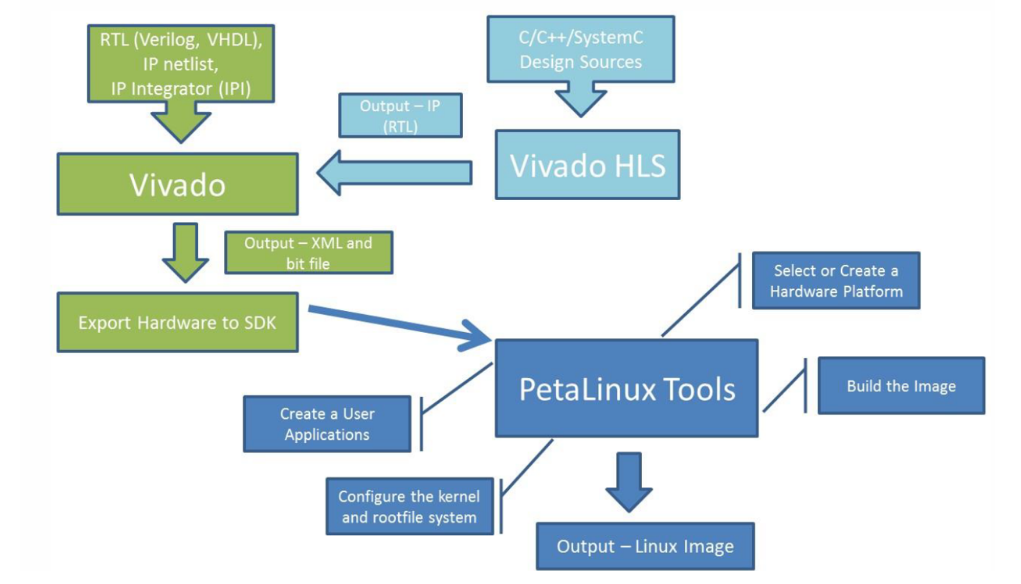
\includegraphics[width=1.1\textwidth]{./images/petalinux-toolflow.jpg}
	\end{center}
	\vspace{-5pt}
	\caption[PetaLinux-Werkzeugfluss]{Überblick über den PetaLinux-Werkzeugfluss [\cite{petailinuxtool}]} % Eckige Klammer (optional): Caption-Text in Abbildungsverzeichnis
	\label{fig:petalinux:tool:flow}
	\vspace{-5pt}
\end{figure}

Wie man in der Abbildung ~\ref{fig:petalinux:tool:flow} sehen kann, ist es möglich, mit Vivado erstellte Hardware-Designs in petalinux zu importieren, einige Anwendungen in petalinux einzubinden und ein Linux-Image zu erstellen.  

\subsubsection{Petalinux Installation}
Wie jedes Build-System benötigt petalinux viele Ressourcen auf Ihrem PC. Um die Kompilierzeit deutlich zu reduzieren, ist es daher sinnvoll, einen Computer mit folgenden Eigenschaften zu verwenden.\cite{Xilinx2020}

\begin{itemize}
	\item 8 GB RAM
	\item 2 GHz CPU-Takt oder gleichwertig
	\item 100 GB freier HDD-Platz
	\item Petalinux unterstützt nur auf Linux Kernel basierte Betriebssysteme. 
	\item PetaLinux-Tools erfordern, dass Ihr Host-System /bin/sh \textbf{bash} ist
\end{itemize}

 Einmal die vorherigen Voraussetzungen erfüllt, kann man also die Installationsdatei von Petalinux unter diesem Link \href{https://www.xilinx.com/support/download/index.html/content/xilinx/en/downloadNav/embedded-design-tools.html}{Petalinux Installer Download}  herunterladen. 
 mit dem \textbf{mkdir} Kommando in Linux kann man ein Petalinux Installation Ornder erstellen, in dem die Installationsdatei dann kopiert wird. mit dem -p Schalter kann den Ordner in einem spezifischen Ordner erstellen.\\
 
\begin{lstlisting}[language=bash]
 	$ mkdir -p /home/<user>/petalinux/<petalinux-version>
\end{lstlisting}

Mit den folgenden Befehlen kann man die Datei ausführbar machen und der Installationsprozess starten.
\begin{lstlisting}[language=bash]
 	$chmod 755 ./petalinux-v<petalinux-version>-final-installer.run
	$./petalinux-v<petalinux-version>-final-installer.run
\end{lstlisting}

\subsubsection{Wichtige Petalinux Kommando}
\begin{itemize}
	\item \textbf{petalinux-create}: Erstellt ein neue Petalinux Projekt. man kann dem Befehl verschiedenen Optionen zuweisen, 
	\begin{itemize}
		\item \textbf{\emph{type}}: definiert den Projekt Type
		\item \textbf{\emph{template}}: Bei der Erstellung des Projekts kann man eine Vorlage definieren. Für das Projekt wurde zynqMP verwendet.
		\item \textbf{\emph{srcuri}}: Hier wird der Pfad zu einem Board Support Package (BSP) angegeben, das zur Erstellung des Projekts verwendet wird. 
		\item \textbf{\emph{name}}: definiert der Name des Projekts. 
	\end{itemize}
	\item \textbf{petalinux-config}: dieser Befehl wird verwendet zur Initialisierung oder Aktualisierung der Hardwarekonfiguration des Projekts oder Konfiguration der Kernel- und/oder Dateisystemeinstellungen. Je nach Anwendung stehen hier auch uns eine Reihe von Konfiguration-Optionen zur Verfügung. Einige davon sind:
	\begin{itemize}
		\item \textbf{\emph{get-hw-description}}: Initialisiert den Petalinux-Projekt mit einem vom Vivado Hardware-description-file(HDF). PetaLinux verwendet HSI-Dienstprogramme, um Informationen über die Hardware aus dieser Datei zu extrahieren, sowie Informationen wie Intellectual property Cores (IP-Cores), Netze, Ports und Schnittstellen, die in anderen Tools wie dem Devicetree-Generator verwendet werden .
		\item \textbf{\emph{-c rootfs}}: Startet das Konfigurations-Menü des Root-Dateisystems.
		\item \textbf{\emph{-c kernel}}: Startet das Konfigurations-Menü des Kernel. 
	\end{itemize}
	\item \textbf{}
	\item \textbf{}
	\item \textbf{}
	\item \textbf{}
	\item \textbf{}
	\item \textbf{}
	
\end{itemize}+